\documentclass{report}
\usepackage{amsmath, amssymb}
\usepackage{tikz}
\usepackage{graphicx}
\usepackage{hyperref}
\usepackage{xcolor}
\usepackage{bm}
\usepackage{mathtools}

\renewcommand{\vec}{\bm}
\newcommand{\uv}[1]{\hat{\bm{#1}}}
\newcommand{\un}{\hat{\bm{n}}}

%\newcommand{\uv}[1]{\hat{#1}}
%\newcommand{\un}{\hat{n}}

\newcommand{\abs}[1]{\left\vert{#1}\right\vert}
\newcommand{\td}[2]{\frac{d{#1}}{d{#2}}}
\newcommand{\std}[2]{\frac{d^2{#1}}{d{#2}^2}}
\newcommand{\pdt}[2]{\frac{\partial{#1}}{\partial{#2}}}
\newcommand{\spdt}[2]{\frac{\partial^2{#1}}{\partial{#2}^2}}
\newcommand{\op}{{\,\prime}}
\newcommand{\tp}{{\,\prime\prime}}
\DeclareMathOperator{\grad}{\nabla}
\DeclareMathOperator{\dive}{\nabla\cdot}
\DeclareMathOperator{\curl}{\nabla\times}

\begin{document}
\tableofcontents
\chapter{Conduction in Semiconductors}\label{c1}
\section{Fermi-Dirac distribution}\label{c1s1}
The Fermi-Dirac distribution function is
\begin{equation}\label{c1e1}
f(E) = \frac{1}{1 + \exp(\frac{E - \mu}{k_BT})},
\end{equation}
where $\mu$ is the chemical potential at $0$ K. If the temperature is slightly
greater than $0$ K, some electrons in the valence band will be excited to the
conduction band, leaving an equal number of holes in the valance band. If $N_v$
and $N_c$ are the density of states in the valence and conduction bands 
respectively then the number density of electrons is
\begin{equation}\label{c1e2}
n = N_c f(E_c)
\end{equation}
At temperature slightly greater than zero, the argument of the exponential is
a very large number and we can as well ignore the $1$ in the denominator of
$f(E_c)$ and write \eqref{c1e2} as
\begin{equation}\label{c1e3}
n = N_c\exp\left(-\frac{E_c - \mu}{k_BT}\right).
\end{equation}
Holes are an absence of electrons. Therefore, the probability distribution of
holes is $f_h(E) = 1 - f(E)$ so that at the top of the valence band
\begin{equation}\label{c1e4}
f_h(E_v) = 1 - f(E_v) = \frac{e^{(E_v - \mu)/k_BT}}{1 + e^{(E_v - \mu)/k_BT}}.
\end{equation}
At temperature slightly greater than zero, the argument of the exponentials is
a large negative number and therefore the denominator almost equal to $1$. The
density of holes is
\begin{equation}\label{c1e5}
p = N_vf_h(E_v) = N_v e^{(E_v - \mu)/k_BT}.
\end{equation}
Since the crystal is electrically neutral, we must have $n = p$ and hence
\[
N_ce^{-(E_c - \mu)/k_BT}  = N_v e^{(E_v - \mu)/k_BT}
\]
from which we have
\begin{equation}\label{c1e6}
\mu = \frac{E_v + E_c}{2} + k_BT\ln\left(\frac{N_v}{N_c}\right).
\end{equation}
At $T = 0$, the chemical potential is the mean of $E_v$ and $E_c$. For a metal
at $0$ K, $\mu = E_F$ the fermi energy. The quantum theory of metals was 
developed before that of semiconductors and prior to  maturing of quantum
statistical mechanics. As a result, the term fermi energy continued to be used
even though there is no fermi surface in a semiconductor. From now one, we will
call $\mu$ the fermi energy $E_F$ and write the distribution function of 
\eqref{c1e1} as
\begin{equation}\label{c1e7}
f(E) = \frac{1}{1 + e^{(E - E_F)/k_BT}} = 
\left[1 + \exp\left(\frac{E-E_F}{k_BT}\right)\right]^{-1}.
\end{equation}

\section{Ge and Si at room temperature}\label{c1s2}
Crystals of pure Si or Ge have a band gap of the $1.21$ eV and $0.785$ eV at
absolute zero. The gap narrows as temperature rises. At $300$ K, it is $1.1$ eV
in Si crystal and $0.72$ eV in Ge. Typical energy at this temperature is $k_BT
\approx 0.025$ eV. It is quite small as compared to the band gap and the 
probability of an electron having enough energy to overcome the band gap is
miniscule. To compute the probability, we need the value of $E_F$ for the two
crystals. There are two ways to compute it:
\begin{itemize}
\item If the energy of an electron just outside the crystal is set to zero 
then all the energies inside the crystal are negative. For an Si crystal,
$E_c = -4.05$ eV, $E_v = -5.17$ eV so that $E_g = -4.16$ eV at absolute zero.
For a Ge crystal, $E_c = -4.00$ eV, $E_v = -4.785$ eV, $E_F = -4.3925$ eV.
\item While working with a single crystal, it is common to let $E_v = 0$ so
that $E_F = E_c/2 = E_g/2$. We will follow this convention.
\end{itemize}

If $E_v = 0$, then the probability of an electron to have energy $E_c$ is
\[
f(E_c) = \frac{1}{1 + e^{E_c/(2K_BT)}} = \frac{1}{1 + e^{E_g/(2k_BT)}}.
\]
At room temperature, the band gap for Ge is $0.72$ eV while $k_BT\approx 0.025$
eV so that the argument of the exponential is approximately $14.4$, allowing us
to write $f(E_c) \approx e^{-E_g/k_BT} \approx 10^{-7}$. With a density of 
states of the order of $10^{19}$ the density of electrons in the conduction band
is approximately $10^{12}$ per cm$^3$. Although this number is small as compared 
to the density of free electrons in a Cu crystal ($\approx 10^{23}$), it is 
enough for Ge to cease to be an insulator and be a semiconductor instead.

For Si crystal at room temperature, $E_g = 1.1$ eV, $E_g/(2k_BT) \approx 22$
and $f(E_c) \approx 10^{-10}$. The density of state is $\approx 10^{19}$ so that
the density of electrons in the conduction band is $\approx 10^9$ per cm$^3$.

\section{Conductivity of a semiconductor}\label{c1s3}
The steady-state velocity of a charge carrier in a crystal is proportional to
the driving field. The constant of proportionality is called the carrier's
mobility. Thus, the drift velocity is
\begin{equation}\label{c1e8}
\vec{v} = \mu\vec{\mathcal{E}},
\end{equation}
where $\vec{\mathcal{E}}$ is the applied electric field. If $n$ is the number density
of the charge carriers then the current density is
\begin{equation}\label{c1e9}
\vec{J} = ne\vec{v} = ne\mu\vec{\mathcal{E}},
\end{equation}
so that from Ohm's law we get an expression for the crystal's conductivity
\begin{equation}\label{c1e10}
\sigma = ne\mu.
\end{equation}

In a semiconductor, there are two types of charge carriers of opposite charges.
An applied electric field drifts them in opposite directions but their current
is in the same direction. As a result, the current density in a semiconductor
crystal is
\begin{equation}\label{c1e11}
J = (n\mu_n + p\mu_p)e\mathcal{E} = \sigma\mathcal{E},
\end{equation}
and its conductivity is
\begin{equation}\label{c1e12}
\sigma = (n\mu_n + p\mu_p)e.
\end{equation}
In these equations, $n$ and $p$ are number densities of electrons and holes and
$\mu_n$ and $\mu_p$ are their mobilities. $-e$ is the charge on the electron.
For a pure, that is undoped, semiconductor crystal, $n = p$ and the common
number is denoted by $n_i$, the intrinsic carrier density. Equation 
\eqref{c1e11} simplifies to
\begin{equation}\label{c1e13}
J = n_i(\mu_n + \mu_p)e\mathcal{E}.
\end{equation}

The common carrier density $n_i$ can be calculated from
\begin{equation}\label{c1e14}
dn_i = N(E)f(E)dE,
\end{equation}
where $N(E)$ is the density of states in conduction band for electrons and
valence band for holes. Electrons in a conduction band can be modelled as
free particles in a box. Let us assumes that the box is a cube of side $L$.
In a stationary state, the electrons will form standing waves with wavelengths
given by
\[
L = n_i\frac{\lambda_i}{2}, i = 1, 2, 3, n_i \in \mathbb{N}.
\]
The momentum components $p_i$ are, therefore, constrained to have values
\[
p_i = \frac{h}{\lambda_i} = n_i\frac{h}{2L}, n_i \in \mathbb{N}.
\]
Thus, every momentum state $(p_1, p_2, p_3)$ occupies a volume $h^3/(8L^3)$ in
the momentum space. Equivalently, the density of states is $8V/h^3$, where
$V = L^3$ is the volume of the box. The number of energy states in a shell of 
radius $p$ and thickness $dp$ is
\[
2 \times 4\pi p^2 dp \times \frac{8V}{h^3} \times \frac{1}{8}.
\]
Here $2$ takes into account the two spin states, $1/8$ is the octant of 
positive integers $n_i$, $4\pi p^2 dp$ is the volume of the shell and $8V/h^3$
is the density of momentum states. Upon simplification, the quantity is
\[
\frac{8\pi p^2}{h^3}dp.
\] 
If $E$ is the energy of the electrons and $m_n$ is their mass
\[
E = \frac{p^2}{2m_n}.
\]
and $N(E)dE$ is the number of energy states per unit volume between $E$ and
$dE$,
\begin{equation}\label{c1e15}
N(E)dE = \frac{4\pi}{h^3}(2m_n)^{3/2}E^{1/2}dE.
\end{equation}
In this analysis, we assumed that the lowest energy is zero. (Although the 
electron never has zero energy.) If the energies start from the bottom of the
conduction band, equation \eqref{c1e15} is modified to
\begin{equation}\label{c1e16}
N(E)dE = \gamma(E - E_c)^{1/2}dE,
\end{equation}
where 
\begin{equation}\label{c1e17}
\gamma = \frac{4\pi}{h^3}(2m_n)^{3/2}.
\end{equation}
Note that $N(E)$ is the density of states. Not all of them will be occupied.
Therefore, the number of charge carries with energy between $E$ and $E + dE$ is
\begin{equation}\label{c1e18}
dn = N(E)f(E)dE
\end{equation}
and the concentration of electrons in the conduction band is
\begin{equation}\label{c1e19}
n = \int_{E_c}^\infty N(E)f(E)dE.
\end{equation}
The energies in the conduction band are much greater than the fermi level so
that $(E-E_F) \gg k_BT$ and we can approximate $f(E)$ as $e^{-(E-E_F)/k_BT}$
so that
\begin{eqnarray*}
n &=& \gamma\int_{E_c}^\infty (E - E_c)^{1/2}e^{-(E - E_F)/k_BT}dE \\
 &=& \gamma e^{-(E_c - E_F)/k_BT} 
\int_{E_c}^\infty (E-E_c)^{1/2}e^{-(E - E_F)/k_BT}dE
\end{eqnarray*}
Since
\begin{equation}\label{c1e20}
\int_0^\infty x^{1/2}e^{-ax}dx = \frac{\sqrt{\pi}}{2a^{3/2}}
\end{equation}
we get
\begin{equation}\label{c1e21}
n =\gamma e^{-(E_c - E_F)/k_BT} \frac{\sqrt{\pi}}{2}(k_BT)^{3/2}
= N_Ce^{-(E_c - E_F)/k_BT},
\end{equation}
where
\begin{equation}\label{c1e22}
N_C = \frac{4\pi}{h^3}(2m_n)^{3/2} \frac{\sqrt{\pi}}{2}(k_BT)^{3/2} = 
2\left(\frac{2\pi m_nk_BT}{h^2}\right)^{3/2}.
\end{equation}

\chapter{The pn junction}\label{c2}
\section{Semiconductor junctions}\label{c2s1}
Metal-semiconductor junctions were known even before the semiconductor diode
became popular. Crystal rectifiers were used in microwave and radio-frequency
electronics even befoce vacuum tube diodes were developed. These junctions were
between crystals of different materials. In this chapter, we will consider a
junction formed by a sharp transition of impurity concentration in a single
crystal. The junction has its origin in the chemical and not mechanical 
inhomogeneity. We will largely follow the treatment in Shockley's 
\cite{shockley1949theory} paper of 1949.

Figure \ref{fig1} shows the schematic diagram of a pn junction, published in
Shockley's paper \cite{shockley1949theory}
\begin{figure}[htbp]
\centering
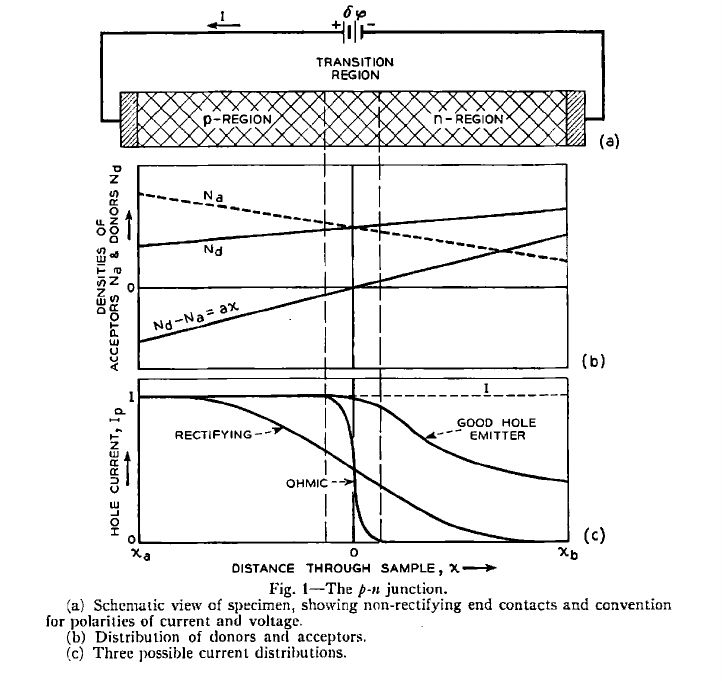
\includegraphics[width=0.95\textwidth]{pn-junction-shockley1949}
\caption{A p-n junction}
\label{fig1}
\end{figure}

The p-side has an excess of acceptor impurity over donor impurity. The situation
is the other way round on the n-side. The junction exists at a point where 
$N_A = N_D$. The concentration $|N_A - N_D|$ is small in a neighbourhood of the
junction, call the \emph{transition layer}. Beyond the transition layer, the
impurity concentration is substantial. 

A rectifying junction is formed when charge carriers diffuse across the 
junction. The electrons diffusing across the junction combine with the holes
resulting in a drop in hole current as we approach the junction. The hole
diffuse across the junction resulting in a decreasing hole current on the
n-side of the junction. Likewise, the electon current starts dropping as we
approach the junction from the n-side and it persists for some distance in the
p-side.

If the junction has many defects or recombination centres then the electrons
diffusing from the n-side are mostly combined with the holes arriving from the
opposite direction in the close vicinty of the junction. There is hardly any
diffusion of minority carriers across the junction. The transition layer is
extremely narrow or non-existent. As a result, when the device is 
reverse-biased, there is a copious generation of electron-hole pairs at the
junction and no drop in current compared to when the device is forward-biased.
Such a junction is a non-rectifying junction.

\section{The transition region}\label{c2s2}
The density of electrons in the conduction band is given by \eqref{c1e3} as
\[
n = N_C e^{-\beta(E_c - \mu)},
\]
where $N_C$ is the density of states, $E_c$ the lowest energy in the conduction
band and $\mu$ is the chemical potential. As long as the doping is not 
excessive, the presence of dopants does not appreciable change the crystal 
structure of the host. As a result, the band structure is unchanged and so is
the density of states. However, the chemical potential shifts because of 
impurities. We observed in equations \eqref{c1e43} (\eqref{c1e44}) that the
presence of donor (acceptor) impurities pushes the chemical potential upwards
(downwards), closer to $E_c$ ($E_v$). In this section, we shall call the 
chemical potential of the intrinsic crystal $\mu_i$. Thus, we have \eqref{c1e13}
for a doped crystal and
\begin{equation}\label{c2e1}
n_i = N_c e^{-\beta(E_c - \mu_i)}
\end{equation}
as its analogue for the pure crystal. Taking their ratio, we get
\begin{equation}\label{c2e2}
\frac{n}{n_i} = e^{-\beta(\mu - \mu_i)}.
\end{equation}
Similarly, for the hole concentration, we have
\begin{equation}\label{c2e3}
\frac{p}{p_i} = e^{-\beta(\mu_i - \mu)}.
\end{equation}
When the crystal is placed in an electric potential $V(x)$, its internal, 
periodic potential shifts by that amount. All energy levels shift. However, 
the differences between them, like the band gap, remain unchanged. We now
choose the zero of our potential at $\mu_i$ so that when we apply the voltage,
the chemical potential of the intrinsic crystal becomes $\mu_i = -eV$, $e > 0$ 
being the elementary charge. If we also write $\mu = -e\varphi$ then equations
\eqref{c2e2} and \eqref{c2e3} become
\begin{eqnarray}
n &=& n_i e^{\beta e(V - \varphi)} \label{c2e4} \\
p &=& n_i e^{\beta e(\varphi - V)} \label{c2e5}
\end{eqnarray}
where we used the fact that $p_i = n_i$ for an intrinsic semiconductor. If
$N_D$ and $N_A$ are the concentrations of donor and acceptors then the total
charge density is
\begin{equation}\label{c2e6}
\rho = e(p - n + N_D - N_A),
\end{equation}
which, using \eqref{c2e4} and \eqref{c2e5} becomes
\begin{equation}\label{c2e7}
\rho = e(N_D - N_A + 2n_i\sinh(\beta e (\varphi - V)).
\end{equation}

There is a further modification to the chemical potential when there is an
injection of carriers or their generation due to other means like light. If
we denote it be $\varphi_n$ and $\varphi_p$ for the electrons and holes
respectively, we get
\begin{eqnarray}
n &=& n_i e^{\beta e(V - \varphi_n)} \label{c2e8} \\
p &=& n_i e^{\beta e(\varphi_p - V)}. \label{c2e9}
\end{eqnarray}
The net hole current is due to diffusion as well as drift. Thus,
\begin{equation}\label{c2e10}
\vec{J}_q = -eD_p\grad{p} - e\mu_p p \grad{V},
\end{equation}
where $D_p$ is the hole diffusion constant and $\mu_p$ is the hole mobility.
From equation \eqref{c2e9},
\[
\grad p = pe\beta(\grad\varphi_p - \grad V)
\]
so that \eqref{c2e10} becomes
\[
\vec{J}_p = -pe^2\beta D_p\grad\varphi_p + pe^2\beta D_p\grad V - 
e\mu_p p\grad{V}.
\]
Using equation \eqref{c1e46}, the last two terms cancel each other and we get
\begin{equation}\label{c2e11}
\vec{J}_p = -e\mu_p p \grad\varphi_p.
\end{equation}
Likewise, we have
\begin{equation}\label{c2e12}
\vec{J}_n = -e\mu_n n \grad\varphi_n = -eb\mu_p n\grad\varphi_n,
\end{equation}
where $b = \mu_n/\mu_p$ is the ratio of the mobility of the two carriers.


\nocite{*}
\bibliographystyle{plain}
\bibliography{basic_devices}
\end{document}  
